\section{Compiler} \label{section:compiler}

Promises\cite{Liskov1988} describes a mechanism to replace RPCs in order to allow concurent parallelism in a distributed system.

They argue that for performance concerns, are better because asynchronous, but harder for the developer to develop.
So their solution is to provide a mechanism allowing asynchronism between the caller and the callee, with a promise about the result of this call for the caller to manipulate the result.

Promises are about distributed system already, it's exactly like fluxions : a system to help the developer abstract parallelism in distributed system, without sacrificing performance.

Futures allow parallelisation of evaluation in a programming language, by stopping processes that need a value not yet ready.

message passing is better for performance, but call is better for human (see Promises: linguistic support for efficient asynchronous procedure calls in distributed systems).

Promises and Futures are a synchronisation mechanism to abstract call into message passing.









Javascript is a functional and dynamically typed language initially introduced to handle user interactions within Web pages.
While Javascript isn't natively event-based, the DOM used in Web pages is.
The latter uses an event-loop to handle events happening on the Web page, and then triggers associated functions the developer provides.
Javascript is not a pure functional language.
As functions have access to the scope of their parents, multiple handlers can share a context.
However, there is no possible concurrence between the handlers as there is only one execution thread.

More recently, \textit{Node.js} used the same event-loop based structure, to propose a non-blocking, event-based execution environment, specifically adapted for real-time I/O intensive applications like Web services.
Because of this event-loop based architecture, the I/O API \textit{Node.js} provides is non-blocking and asynchronous.
The invocation of any function from this API returns immediately not to block the execution with time consuming I/O operations.
The last argument provided by the developer to this function must be a handler function to invoke when the operation completes.
This function is commonly named a callback.
The \textit{Node.js} event-loop receives and gathers every I/O event, waiting its turn in the loop to invoke the associated callback.
Listing \ref{lst:callback} illustrates the call of the asynchronous function \texttt{asyncFn} with the callback \texttt{callbackFn}.

\begin{code}[Javascript, caption={Example of an asynchronous function call},label={lst:callback}]
function MyFn() { 
  var a = 1,@\Comment{\circled{1}}@
      b = 2,
      c = 3;
  asyncFn(a, b, function callbackFn(result) {
    // process the result of asyncFn @\Comment{\circled{3}}@
    // Use variables b, and c.
  });
  // result is not yet ready @\Comment{\circled{2}}@
}
\end{code}

\begin{figure}[h!]
  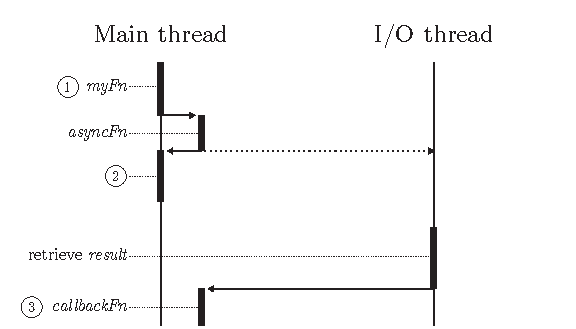
\includegraphics[width=\linewidth]{callback.pdf}
  \caption{Illustration of listing \ref{lst:callback}}
  \label{fig:callback}
\end{figure}

In most imperative languages the execution is synchronous by default, while special libraries handle parallelism, some using asynchronism and callbacks\cite{Liskov1988}.
However, Node.js imposes natively both synchronous and asynchronous paradigms, as seen above, listing \ref{lst:callback}.
The invocation of \texttt{asyncFn}, \circled{3}, and the code following the invocation, \circled{2}, are independent from each other because the execution order isn't deterministic.
This invocation of an asynchronous function virtually splits the execution and create a possible parallelism between these two execution paths.
Because of the parallelism implied by this independence, we think it is possible to isolate these parts enough to encapsulate them in fluxions, and migrate their execution onto different machines.
Figure \ref{fig:callback} illustrates the two isolated parts encapsulated in fluxions from listing \ref{lst:callback}.

\begin{figure}[h!]
  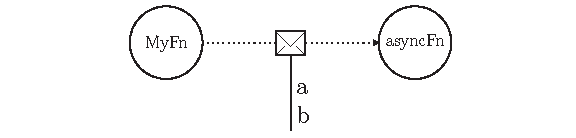
\includegraphics[width=\linewidth]{callbackFlx.pdf}
  \caption{Illustration of listing \ref{lst:callback} broken into fluxions}
  \label{fig:callback}
\end{figure}

In the next subsections, we describe our work on a compiler to break a program into many independent parts and enclose them in fluxion.
We then address the limitations of this method, and possible future improvements.

\subsection{Breaking the program}

As asynchronous functions indicates frontier along which the program is breakable into independent parts, the very first step of the compilation process is to spot them by analyze of the source code.
We statically analyze the source code using an intermediate representation of it : the Mozilla Javascript Abstract Syntax Tree (AST)\footnote{\raggedright https://developer.mozilla.org/en-US/docs/Mozilla/Projects/SpiderMonkey/Parser\_API}.
This structured representation breaks the source into a tree of nodes, each representing a construct from the source, like an operation or an identifier.
It can be traversed and allow easy modification of its structure, without the risk of errors involved by direct source manipulation.
In an AST, the node of a function call is of type \textit{CallExpression}, and contains a reference to the callee and an array of the arguments.
As an asynchronous function call marks the frontier between two fluxions, most modifications required to split the execution paths happen around the nodes of this type.

We distinguish two types of asynchronous functions in the \textit{Node.js} I/O API : the functions handling a series of I/O events, and the functions handling only one I/O event.
We details in the next paragraphs how the compiler modify these two types of asynchronous functions.
We explain in section \ref{ss:Limitations} why the compiler needs a list of asynchronous function with their type to distinguish between the two types.

\subsubsection{Series of events} \label{sss:start}

Some asynchronous functions provide a callback for a series of future event.
Like the function \texttt{app.get} from listing \ref{lst:classique}, line \ref{lst:classique_get}.
The callbacks of these functions indicate the input of a data stream in the program, and the beginning of a fluxions chain.
As the callbacks mark the frontier between the current fluxion and the beginning fluxions chain, the compiler replaces the callback by a placeholder function starting the chain.
This placeholder function uses the function \texttt{start(<msg)} provided by the fluxionnal execution model described section \ref{section:model}.
The placeholder function is detailed later, section \ref{ss:Scope}.

Algorithm \ref{alg:CallExpressionStart} details the \texttt{StartCallExpression} function called while walking the AST to do the callback replacement.
On line number \ref{alg:CallExpressionStartCreateFluxion}, it creates the first fluxion of the chain to include the callback previously parsed.
On line number \ref{alg:CallExpressionStartPlaceholder}, the callback is replaced with a placeholder function.

\begin{algorithm}
\caption{Algorithm to replace callback from start function call}
\label{alg:CallExpressionStart}
\begin{algorithmic}[1]
\Function{StartCallExpression}{\null}
\For{$argument$ \textbf{in} $arguments$}
\If{$argument$ is a Function}
\State $argument.name + unique identifier \to name$
\State Create fluxion $name$ parsing $argument$ \label{alg:CallExpressionStartCreateFluxion}
\State Register output to $name$
\State $placeholder \to argument$ \label{alg:CallExpressionStartPlaceholder}
\EndIf
\EndFor
\EndFunction
\end{algorithmic}
\end{algorithm}

\subsubsection{One-time event} \label{sss:post}

The other type of asynchronous functions provides immediate I/O operation.
Callbacks of these functions are invoked only once, and continue the execution after the completion of the I/O operation.
Because of their asynchronism, these function calls mark the frontier between the current fluxion and the next one, inside a chain of fluxion.
The compiler replaces the asynchronous function call by a call to a placeholder function.
This placeholder function uses the function \texttt{post(<msg>)} provided by the fluxionnal execution model described section \ref{section:model}.
The placeholder function is detailed later, section \ref{ss:Scope}.

Algorithm \ref{alg:CallExpressionPost} details how the \texttt{PostCallExpression} function replace the asynchronous function call.
Line number \ref{alg:CallExpressionPostCreateFluxion}, the compiler parses the current node containing the \textit{CallExpression} to create the next fluxion.
It creates the next fluxion enclosing the asynchronous function call into a simple function together with the callback declaration.
Callbacks declared \textit{in situ} in the arguments are trivially spotted.
However to accurately detect every callbacks, the compiler needs to track and resolve every identifier used in the program to identify their type.
We address the problem of unresolvable callbacks in section \ref{ss:Limitations}.
On line number \ref{alg:CallExpressionPostPlaceholder}, a placeholder function call replace the asynchronous function call.
This placeholder is invoked instead of the asynchronous function and sends a message to the next fluxion.

\begin{algorithm}
\caption{Algorithm to replace post function call}
\label{alg:CallExpressionPost}
\begin{algorithmic}[1]
\Function{PostCallExpression}{$node$}
\If{$node.callee$ is asynchronous}
\State $node.callee.name + unique identifier \to name$
\State Create fluxion $name$ parsing $node$ \label{alg:CallExpressionPostCreateFluxion}
\State Register output to $name$
\State $placeholder \to node$ \label{alg:CallExpressionPostPlaceholder}
\EndIf
\EndFunction
\end{algorithmic}
\end{algorithm}

These two compilation algorithms break the program into fluxions, and register the inputs and outputs of each to build a network map of the program.
The compiler uses this map to resolve the remaining dependencies between this parts.
We address in the next section this dependencies problem, as well as the placeholder function.

\subsection{Scope sharing and Concurrency} \label{ss:Scope}

In Javascript, each function create a new scope containing variables local to itself.
This scope is chained to the scope of the parent function, so that the child function can access the scope of the parent.
Callbacks defined inside a scope can access the same scope as the calling function, allowing them to share variables even while their executions are asynchronous.
As an example, in listing \ref{lst:callback}, \texttt{callbackFn} is defined inside \texttt{MyFn}, so it can access \texttt{MyFn}'s scope containing variables \texttt{a}, \texttt{b} and \texttt{c}.
By isolating a callback, we break its dependencies with its parent scope. These needs to be resolved.

While walking the AST, the compiler register and track every use of variables to determine which ones and what type of access the fluxion needs, and which scope they belong to.
This set of variables needed by a fluxion represent its signature.
For example, the signature of the fluxion created out of \texttt{asyncFn}, listing \ref{lst:callback} include variables \texttt{b} and \texttt{c} as they are used in \texttt{callbackFn}, as well as \texttt{a} because it is used by the function call to \texttt{asyncFn}.
To resolve these dependencies, during the execution, the parent function sends the signature of the next fluxion in the same message together with the result of the asynchronous operation.
As the placeholder function call have the same scope than the asynchronous function call or callback it replaces, it is responsible for gathering the variables from the signature in a message along with the result of the operation and send it to the next fluxion.
The placeholder function call replacing \texttt{asyncFn} after compilation of listing \ref{lst:callback} is described in listing \ref{lst:placeholder}, line \ref{lst:placeholdercall}.

\begin{code}[Javascript, caption={Example of a placeholder function call},label={lst:placeholder}]
function MyFn() {
  var a = 1,
      b = 2,
      c = 3;

  // Placeholder for asyncFn-uid
  flx.post(flx.m("asyncFn-uid", {a, b, c})); @\label{lst:placeholdercall}@
}
\end{code}



% Stream line
As fluxions are chained one after another, a fluxion must provide every dependency for the next one, even if some of this dependencies miss from its own scope or signature.
These dependencies must be passed fluxion after fluxion from the producing fluxion, to the consuming fluxion.
So, the message stream linking one fluxion to another includes the signature of the next fluxion as well as dependencies targeting downstream fluxions.
The compiler has to resolve the content of these message streams beginning by the last fluxions and going upstream to the first ones.
Figure \ref{fig:streamline} illustrate this principle : since fluxion \textit{C} needs the variable \textit{z}, fluxion \textit{B} needs the variable \textit{z} as well to pass it along to fluxion \textit{C}.

\begin{figure}[h!]
  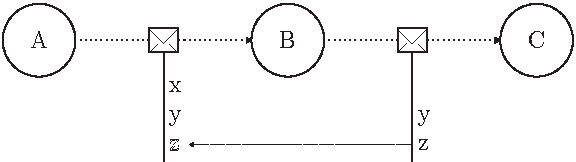
\includegraphics[width=\linewidth]{streamline.pdf}
  \caption{Fluxion C needs the variable z, so does fluxion B}
  \label{fig:streamline}
\end{figure}

\subsection{Limitations} \label{ss:Limitations}

\textit{Node.js} uses the convention to place the callback as the last parameter.
While most of the \textit{Node.js} API is asynchronous and uses this convention, Javascript allows to pass a function as an argument whether the callee is asynchronous or not.
For example, functions from the \texttt{Array} prototype ask functions as parameters for a behavior to call on each iteration over the array.
Listing \ref{lst:array} presents an example of this structure.
This iteration is synchronous, so the function passed as an argument, \circled{1}, and the code following the function call, \circled{2}, are somehow dependent.
Leaving an asynchronous function call as is doesn't introduce bugs, however breaking a synchronous function by replacing its callback leads to bugs.
To avoid introducing new bugs, it is important for the compiler to be able to distinguish between these synchronous and asynchronous functions.

\begin{code}[Javascript, caption={Example of a synchronous function using a callback},label={lst:array}]
  my_modified_array = my_array.map(function(element) {
    // Modifying element @\Comment{\circled{1}}@
  })
  // Following code @\Comment{\circled{2}}@
\end{code}

The compiler is unable to distinguish by itself between the synchronous and asynchronous functions, or between the two types of asynchronous functions described in section \ref{sss:start} and \ref{sss:post}.
We propose to provide for the compiler a list of every asynchronous function likely to be broken into fluxions, with their type specified.
With this list, the compiler is able to modify asynchronous functions accordingly to their type, while leaving untouched every other function.

Even synchronous, the use of a callback by the \texttt{map} function indicate an independence between the callback and the main execution thread.
For future improvements, we focus on studying these independences to allow the compiler to spot and break into fluxions these patterns of synchronous function call using callbacks.

% Problem with dynamically typed functions

% Functions are of higher order in Javascript, so arrays can contain functions, as well as a variables.
Javascript is dynamically typed, if the index to access an array can't be resolved statically, then so do the type of the result.
Some callbacks can't be resolved statically.
For example, in listing \ref{lst:unresolved}, the function \texttt{myAsyncFn} is asynchronous and ask for a callback as parameter.
The compiler would break the program along its call, however \texttt{event.type} is unresolvable statically, the compiler is unable to include the callback in the next fluxion.
This structure might already be encapsulated inside a fluxion, and the callback might need variables from the scope of an upstream fluxion, but as the callback is unresolved, it is impossible for the compiler to track them, and add these dependencies in the signature of the current fluxion.
Even if the compiler leaves this structure as is, it introduce dependency bugs as the compiler is unable to resolve dependencies and generate accurate signatures.
The compiler is currently unable to compile a program containing structures involving dynamic resolution like in listing \ref{lst:unresolved}.

\begin{code}[Javascript, caption={Example of an unresolvable callback},label={lst:unresolved}]
myHandlers = [];
// ... definition of myHandlers
onEvent(function(event) {
  myAsyncFn(myHandlers[event.type])
})
\end{code}

For future improvements, we focus on a solution to dynamically compile fluxions and resolve dependencies, allowing to compile programs containing dynamic structures described in the last paragraph.

\subsection{Compilation example}

As of today our work on the compiler is still incomplete, there is inconsistencies between the high-level language detailed in section \ref{section:model} and the compilation results.
For documentation purposes, this section details the compiler current state of progress.

Listing \ref{lst:compsource} is a simplified version of the example listing \ref{lst:classique} in section \ref{section:model}.
We use this simplified version as a test for our compiler, as it is yet unable to handle dynamic resolution, like used with the object \texttt{count} line \ref{lst:classique_dynres} in listing \ref{lst:classique}.
The result of this compilation is listing \ref{lst:comptarget}.
In the compilation result, the fluxion \textit{id-1000} should hold a context containing the variable \texttt{count}, like the object \texttt{uid} in the context of fluxion \textit{logic}, listing \ref{lst:fluxionnal}.
But our compiler is yet unable to correctly resolve dependencies and fluxion contexts, so this counter service is unable to increment visits.

\begin{code}[Javascript, caption={Simplified version of the initial service},label={lst:compsource}]
var app = require('express')();
var count = 0;

app.get("/:id", function id(req, res){
  count = count + 1;
  res.send(count);
});

app.listen(8080);
\end{code}

\begin{code}[Javascript, caption={Compilation result of code listing \ref{lst:compsource}},label={lst:comptarget}]
// Main >> id
  var flx = require('fluxion');
  var app = require('express')();
  var count = 0;
 
  app.get("/:id"n function placeholder(req, res) {
    flx.start(flx.message("id-1000", {
      res: res,
      count: count
    }))
  })
 
  app.listen(8080);

// id-1000
  flx.register("id-1000", function id-1000(msg){
    res.send(msg.count = msg.count + 1);
  })
\end{code}





